\documentclass[runningheads]{llncs}

\usepackage{graphicx}
\graphicspath{{./figs/}}

\usepackage{amsmath} 
\usepackage{bm}
\usepackage{amsbsy} 
\usepackage{amssymb}
\usepackage{cite}
\usepackage{multirow}

\begin{document}
%
\title{Multiscale model reduction for neutron diffusion equation}
%
%\titlerunning{Abbreviated paper title}
% If the paper title is too long for the running head, you can set
% an abbreviated paper title here
%
\author{A.O. Vasilev\inst{1} \and 
D.A. Spiridonov\inst{1} \and
A.V. Avvakumov\inst{2} }
%
\authorrunning{A.O. Vasilev, D.A. Spiridonov \and A.V. Avvakumov}
% First names are abbreviated in the running head.
% If there are more than two authors, 'et al.' is used.
%
\institute{North-Eastern Federal University, Yakutsk, Russia \and
National Research Center \emph{Kurchatov Institute}, Moscow, Russia\\
\email{haska87@gmail.com}
}
%
\maketitle              % typeset the header of the contribution
%
\begin{abstract}
Construction of multiscale method for neutron diffusion equation is provided. 
The neutron diffusion approximation is mostly used for reactor analysis and applied in most engineering calculation codes. 
The solution method is based on the use of a generalized multiscale finite element method.
The main idea is to create multiscale basis functions that can be used to effectively solve on a coarse grid.
Numerical results show that multiscale basis functions can well take into account the small-scale characteristics of the medium and provide accurate solutions. 

\keywords{parabolic equation \and neutron diffusion \and multiscale simulation \and generalized multiscale finite element method (GMsFEM)}
\end{abstract}

\section{Introduction}
Among the basic physical processes occurring in a nuclear reactor \cite{Duderstadt1976}, the focus is on neutron transport. 
To describe that process, a rather complex integro-differential equation is involved, in which the neutron flux distribution depends on time, energy, spatial and angular variables \cite{Stacey2007}.
In practical calculations of nuclear reactors, as a rule, simpler systems of equations in the multigroup diffusion approximation are used. 
The computational model is a system of coupled second-order parabolic equations, which is supplemented by a system of ordinary differential equations to take into account delayed neutrons.

Real dynamic neutronic calculations require the use of large computational grids for large characteristic times. 
Because of this, the computation of the solution can be very expensive.
When solving these problems, it is common to use numerical averaging techniques or different multiscale methods that can significantly reduce the number of unknowns, through the construction of coarse-scale model.
Also note a class of methods for modeling the nonstationary group neutron diffusion, which is associated with the multiplicative representation of the space-time factorization methods and the quasistatic method \cite{dulla2008quasi}. The general strategy for the approximate solution of nonstationary problems of neutron transport, which is oriented to fast calculations using the state change modal method was formulted in \cite{Progress18}.

Homogenization or numerical homogenization methods construct the approximation of the solution on a coarse grid and allow calculating the effective properties of the material.
As a result, the methods of numerical homogenization give macroscopic laws and parameters on the basis of local computations, but such approaches are usually based on a priori formulated assumptions, see e.g. \cite{Stalnov2017,Bakhvalov2012}. 
On the other hand, multiscale methods construct multiscale basis functions in each coarse-grid block and couple these basis functions in a global formulation. 
These methods have a two-way information exchange between micro and macro scales. 
There are many variations of multiscale finite element methods (MsFEM).
A detailed description of several variations of the method is presented in \cite{Efendiev2009}.

In this paper, we consider the solution of the neutron diffusion equation uses Generalized Multiscale Finite Element Method (GMsFEM). 
The main idea of the GMsFEM is to reduce the dimension of the problem. 
GMsFEM  involves two basic steps: (a) the construction of multiscale basis functions that take into account small scale heterogeneities in the local domains and (b) the construction of the coarse scale approximation. 
For the construction of the multiscale basis functions we solve spectral problems in local domains.
Spectral problems help to identify the most important characteristics of the solution. 
In contrast to the available techniques, this method allows to avoid the limitations associated with idealization and limitations on the applicability of the method.
This method also more general technology that takes into account the different scale processes.
The construction of basis functions occurs independently for each local domain, doesn't require the exchange of information between processors, and  has a high parallelization efficiency.
%Basis functions are designed to capture the multiscale features of the solution. 
%Important multiscale features of the solution are incorporated into localized basis functions which contain information about the scales that are smaller (as well as larger) than the local numerical scale defined by the basis functions. 
%The computation of basis functions use local spectral problems to reduce the dimension of the local problem. 

In this paper, we present numerical results for 2D small PWR test. 
We compare GMsFEM results with the fine-grid simulations. 
In our numerical results, we select different number of multiscale basis functions in each local subdomains and show that as we increase the number of basis functions, the multiscale solution becomes more accurate. 
In particular, the results with very few basis functions are not accurate, which indicates that one needs to select more basis functions. 
The error of the method in $L_2$ and $H_1$ norms are shown. 

\section{Problem statement}
Let's consider modelling neutron flux in a one-group diffusion approximation. 
Neutron flux dynamics is considered within a bounded 2D domain  $\Omega$ ($\bm x = \{x_1, x_2\} \in \Omega$) with a convex boundary $\partial \Omega$. 
The neutron diffusion is described by the following set of equations with one group delayed neutron source:
\begin{equation}\label{1}
\begin{split}
 \frac{1}{v} \frac{\partial \phi}{\partial t} - \nabla \cdot D \nabla \phi + \Sigma_r \phi &= \frac{1 - \beta}{K_{eff}} \nu \Sigma_f \phi + \lambda c, \\
\frac{\partial c}{\partial t} + \lambda c &= \frac{\beta}{K_{eff}} \nu \Sigma_f \phi.
\end{split}
\end{equation} 
Here $\phi(\bm x,t)$ --- neutron flux  at point $\bm x$ and time $t$,
$v$ --- effective velocity of neutrons,
$D(\bm x)$ --- diffusion coefficient, 
$\Sigma_r(\bm x,t)$ --- removal cross-section,
$\Sigma_f(\bm x,t)$ --- generation cross-section,
$\beta$ --- effective fraction of delayed neutrons, 
$\lambda$ --- decay constant of sources of delayed neutrons.
System of equations (\ref{1}) is supplement with boundary condition and  initial condition.

The albedo-type conditions are set at the boundary of the area $\partial \Omega$:
\begin{equation}\label{2}
 D\frac{\partial \phi}{\partial n} + \gamma \phi = 0,
\end{equation} 
where $n$ --- outer normal to the boundary $\partial \Omega$, $\gamma$ --- albedo constant.
Let's propose that in the initial time moment (at t = 0) the reactor is in the critical state
\begin{equation}\label{3}
 \phi(\bm x,0) = \phi^0(\bm x).
\end{equation} 
%Let's consider problem (\ref{1}) with boundary conditions (\ref{2}) and initial conditions

To solve the problem in computational domain $\Omega$, we approximate the system of equations (\ref1)-(\ref{3}) using the finite element method.
We discretize the time derivatives using finite-difference scheme, and then bring each stationary problem to a variational formulation. 
For approximation in time, we use a purely implicit scheme with time step $\tau$. 
To specify the variational formulation, we multiply equations by the test function $q$ and integrate over the domain $\Omega$. 
Using the integration by parts, we obtain the following variational formulation: find $\phi^{n+1} \in V$ such that
\begin{equation} \label{4}
\begin{split}
\int_\Omega \frac{1}{v} \frac{\phi^{n+1}}{\tau} q d\bm x +
\int_\Omega D^{n+1} \nabla\phi^{n+1} \cdot \nabla q d\bm x &+ 
\int_\Omega \Sigma_r^{n+1} \phi^{n+1} q d\bm x - \\
\int_\Omega \frac{1+\lambda\tau-\beta}{K_{eff}(1+\lambda\tau)} \nu \Sigma_f^{n+1} \phi^{n+1} q d\bm x &+
\int_{\partial \Omega} \gamma \phi^{n+1} q d\bm s = \\
\int_\Omega \frac{1}{v} \frac{\phi^{n}}{\tau} q d\bm x +
\int_\Omega \frac{\lambda c^n}{1+\lambda\tau} q d\bm x &, \quad \forall q \in V,
\end{split}
\end{equation}
where $V=H^1(\Omega)$ --- sobolev space consisting of scalar functions $\upsilon$ such that $\upsilon^2$ and $|\nabla \upsilon^2|$ have a finite integral in $\Omega$.

Further, it's necessary to pass from the continuous variational problem (\ref{4}) to the discrete problem. 
We introduce finite-dimensional space of finite elements $V_h \subset V$ and formulate a discrete variational problem. 
%We use standard linear basis functions as basis functions to solve the problem on the fine grid and
%\[
%\phi = \sum_{i = 1}^{N_f} \phi_i y_i,
%\] 
%where $N_f$ is the nunber of vertices on the fine grid.

The problem is solving a system of linear algebraic equations
\begin{equation}\label{5}
A_f \phi = b_f,
\end{equation}
where the operator $A_f$ corresponds to the left side of equation (\ref{4}), and the vector $b_f$ corresponds to the right side of equation (\ref{4}).

\section{Multiscale method}
For the discretization on the coarse grid we use GMsFEM.
We construct two grids: fine grid ($\mathcal{T}_h$) and coarse grid ($\mathcal{T}_H$) (see Figure \ref{p1}). 
For multiscale basis construction, we define local domains $\omega_i$, where $i = 1,...,N_v$ and $N_v$ is the number of coarse grid nodes.
We assume that $\mathcal{T}_h$ is a refinement of $\mathcal{T}_H$, where $h$ and $H$ represent the fine and coarse mesh sizes, respectively. 
We assume that the fine-scale mesh $\mathcal{T}_h$ is sufficiently fine to fully resolve the small-scale information of the domain  while $\mathcal{T}_H$ is a coarse mesh containing many fine-scale features.
A local domain $\omega_i$ is obtained by the combining all the coarse cells around one vertex of the coarse grid. 

\begin{figure}[h!]
\centering

\includegraphics[width=0.26\linewidth]{coarse_grid.png}
\hspace{2em}
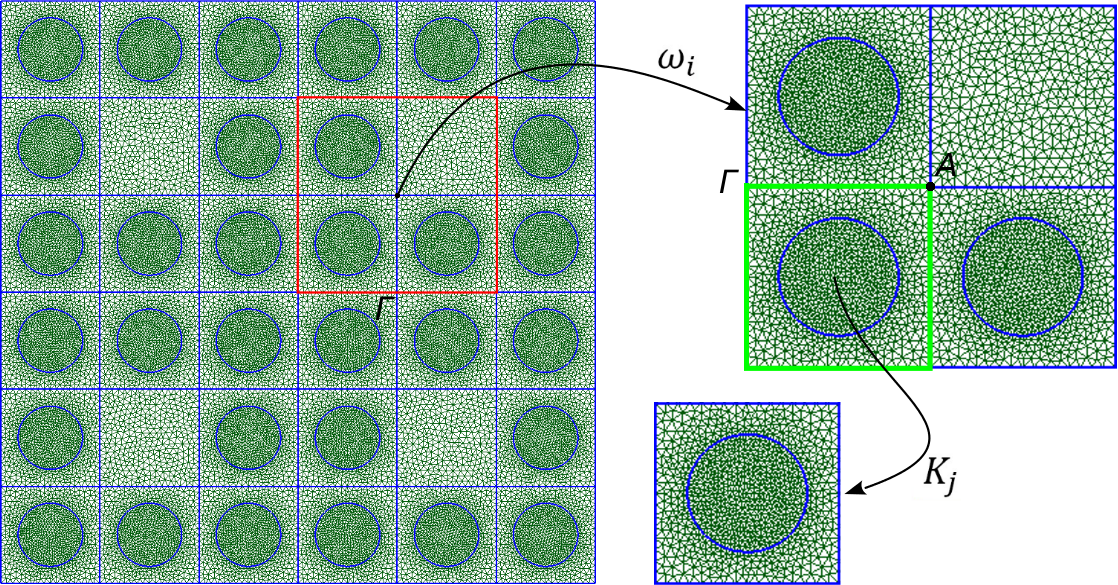
\includegraphics[width=0.5\linewidth]{omega_GA.png} 
\caption{Coarse grid and local domain $\omega_i$ with $K_j$}
\label{p1}
\end{figure} 

Using constructed multiscale basis functions, we construct a mathematical model on a coarse grid that allows to significant reduce the solution time, the amount of used memory, and can be used to perform calculations for a given configuration of  heterogeneous properties. 
We construct the mutiscale function space
\[
{V}_{\text{off}} = \mbox{span} \{ y_j \}_{j=1}^{N},
\]
where $N$ is the number of coarse basis functions.
Each $y_j$ is supported in local domain $w_i$.

% spectral
\textbf{Multiscale space.}
The firts step is the solution of local spectral problems on the local domains.  
In order to construct a conforming basis functions, we multiply eigenvectors related to the smallest eigenvalues to the partition of unity functions.
We use following spectral problem in $\omega_i$
\begin{equation} \label{6}
A \varphi^i = \lambda S \varphi^i,
\end{equation} 
where the elements of the matrices $A= \{ a_{ij} \}$ and $S = \{ s_{ij} \}$ are defined as follow{
\begin{equation} \label{7}
\begin{split}
a_{ij} = 
\int_{\omega_i} D \nabla\phi \cdot \nabla q d\bm x &+ 
\int_{\omega_i} \Sigma_r \phi q d\bm x - 
\int_{\omega_i} \frac{1+\lambda\tau-\beta}{K_{eff}(1+\lambda\tau)} \nu \Sigma_f \phi q d\bm x, \\
s_{ij} &= \int_{\omega _i} D u q d\bm x.
\end{split}
\end{equation}}

{Then, we choose eigenvectors corresponding to the smallest $M_{i}$ eigenvalues from \eqref{6} and use them for the construction of multiscale basis functions.} 

% POU
\textbf{Partirion of unity functions. } As  partition of unity functions, we use linear functions in each domain $\omega_i$.
Partitions of unity are calculated in the domain $ K_j $ as a linear function from $\Gamma$ to the vertex $ A $, and $ 0 $ is assigned to the entire segment $\Gamma$, and at point $ A $ is assigned the value $1$ (see Fig \ref{p1}). 
Thus, we obtain a linear function from $ 0 $ to $ 1 $ over the entire domain $ K_j $. 
%Partitions of unity are shown in Figure \ref{p2}. 
%Domain $K_j$  is one element from a coarse grid. 
%
%\begin{figure}[h!]
%%\centering
%%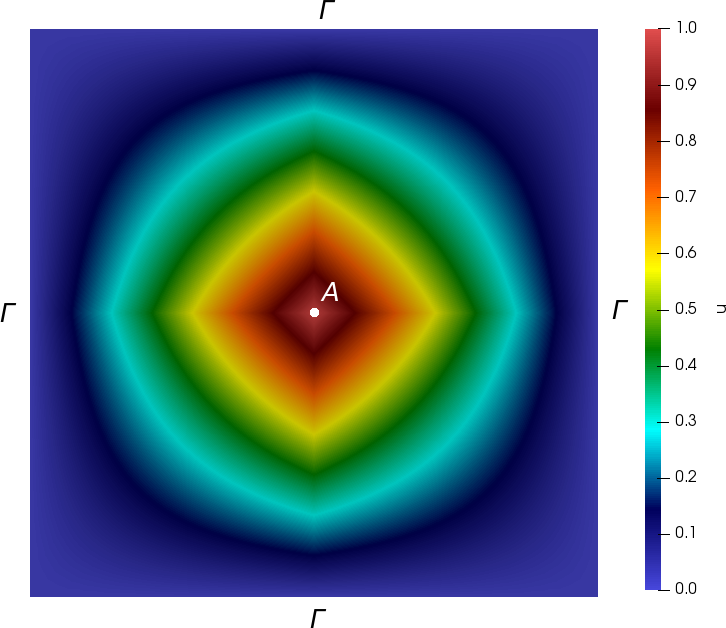
\includegraphics[width=0.3\linewidth]{pofs.png} 
%%\hspace{2em}
%%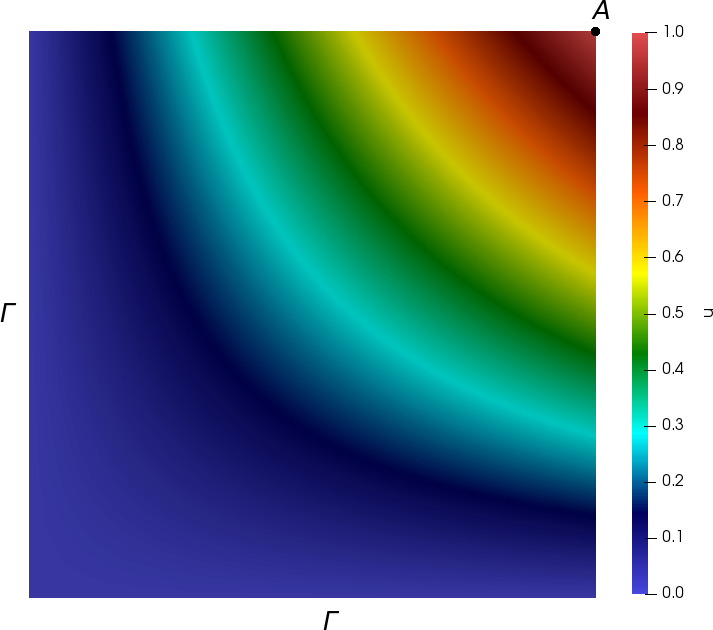
\includegraphics[width=0.3\linewidth]{pouK.png} 
%%\caption{Partirion of unity functions on the $\omega_i$ (right) and $K_j$ (left)}
%%\label{p2}
%\end{figure} 
 
The multiscale space is defined as the span of $y_i = \chi_i \varphi^i_k$, where $\chi_i$ is the usual nodal basis function for the node $i$ (linear partition of unity functions). 
The number of bases can be different, the accuracy of the solution can be improved when we increase the number of bases.

%\subsection{Assembling a matrix in a multiscale space}
\textbf{Coarse-scale approximation. }
Next, we create following  matrix for each $\omega_i$
\[
R^i = \left[ y_1, \ldots, y_{M_i-1},  y_{M_i} \right].
\]
and  define a transition matrix from a fine grid to a coarse grid to reduce the dimension of the problem
\[
R = [ R^1, R^2, ..., R^{N_v} ],
\]
where $N_v$ is the number of local domains $\omega_i$.

Then using transition matrix $R$ and fine grid system (\ref{5}), we construct coarse grid approximation
\begin{equation}\label{9}
A_c \phi_c = b_c, \quad 
A_c = R A_f R^T 
\quad \text{ and } \quad 
b_c = R b_f,
\end{equation}  
and using coarse-scale solution $\phi_c$, we can  reconstruct a fine grid solution $\phi_{ms} = R^T \phi_c$.

\section{Numerical results}
The test problem for reactor small PWR-2D ($\Omega$ --- reactor core area) is considered. 
The geometrical model of the small PWR-2D reactor core is presented in Fig.\ref{p3}. 
The diameter of the fuel rods is 0.82 cm, the cell width is 1.26 cm.
Diffusion neutronics constants in the common notations are given in Table \ref{t1}. 
%There are two types of cassettes, with fuel 1\% $UO_2$ and 2\% $UO_2$.
The boundary conditions (\ref{2}) are used at $\gamma = 0$ (total reflection).
The following delayed neutrons parameters are used: $\beta = 6.5 \cdot 10^{-3}$, $\lambda = 0.08$ s$^{-1}$ and $v = 5 \cdot 10^5$ cm/s.

\begin{figure}[h]
  \begin{center}
    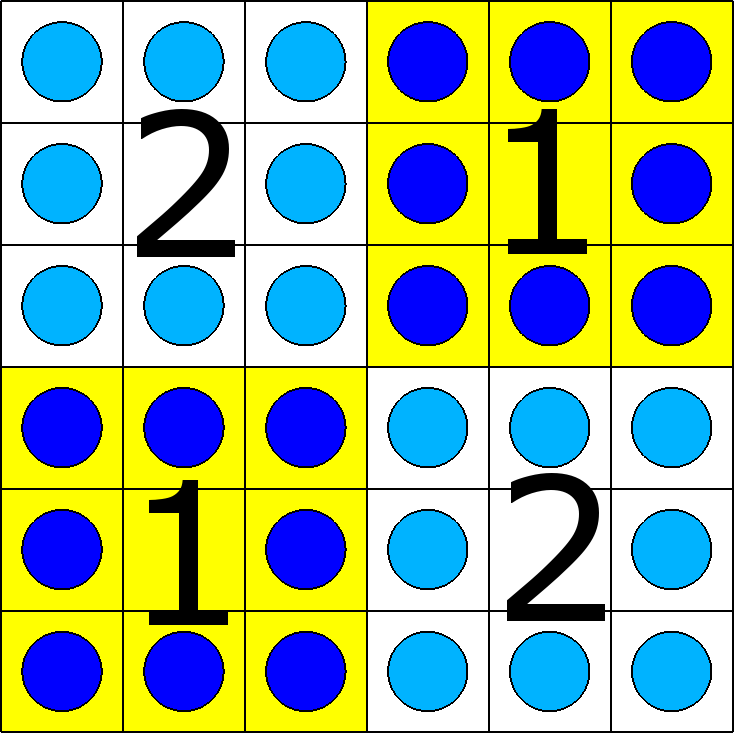
\includegraphics[width=0.4\linewidth] {smallpwr.png}
	\caption{Geometrcial model of the small PWR-2D reactor core}
	\label{p3}
  \end{center}
\end{figure} 

We define the next scenario of the process: The $\lambda$-spectral problem (see \cite{Annals17}) is solved, the solution is taken as the initial condition; 
Calculation for the non-stationary model at the time range 0 to 0.4 sec;
At a moment of 0.1 sec and 0.3 sec the fuel value $\Sigma_a$ for the zone 1 changes to +2\% and -3\% respectively (modeling effect of insertion or withdrawal of control rods).
At each time the integrated power is calculated 
\[P(t) = a\int_{\Omega}\Sigma_f \phi d\bm x,\]
where $a$ is the normalization coefficient by a given value of the integrated power.

\begin{table}[h]
\caption{Diffusion neutronics constants for IAEA-2D test problem}
\label{t1}
\begin{center}
\begin{tabular}{|c|c|c|c|c|c|}
\hline
\multirow{2}{*}{Zone} & \multicolumn{2}{c|}{1} & \multicolumn{2}{c|}{2} \\
\cline{2-5}
& coolant & fuel & coolant & fuel \\
\hline
$D$ & 0.34473872445 & 0.77002585054 & 0.31679441560 & 0.80236505122 \\
$\Sigma_a$ & 5.3858400E-03 & 8.9337900E-02 & 6.0670900E-03 & 6.6279500E-02 \\
$\Sigma_{f}$ & 0.0 & 5.4731800E-02 & 0.0 & 3.3377700E-02 \\
$\nu$ & 0.0 & 2.44844861671 & 0.0 & 2.45482762443 \\
\hline
\end{tabular}
\end{center}
\end{table}

Coarse mesh contains $49$ vertices.
The fine grid contains 115891 vertices. 
The time step for both grids is $\tau = 0.001$.
As an exact solution, we take the solution by the finite element method on a fine grid.
The initial value of $K_{eff}$ was 1.183280. 

\begin{figure}[h!]
\centering
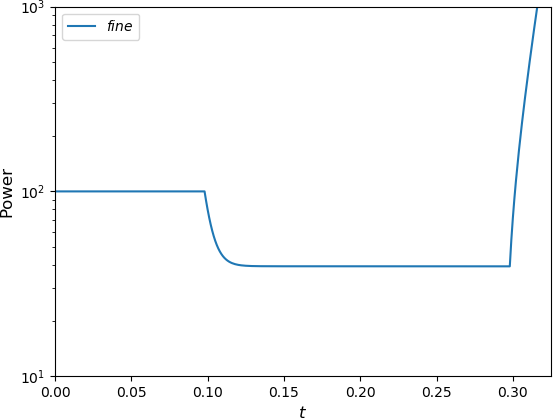
\includegraphics[width=0.45\linewidth]{power_fine.png} 
\hspace{2em}
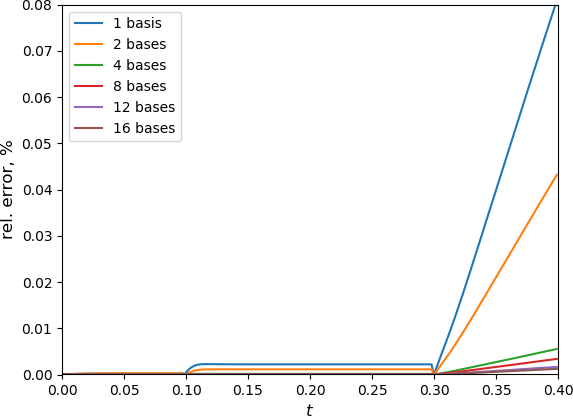
\includegraphics[width=0.45\linewidth]{power.png} 
\caption{Interal power on a fine grid and relative errors ($\%$) of the multiscale solution power.}
\label{p4}
\end{figure}
 
The integral power on a fine grid and relative errors of a integral powers for multiscale soultion shown in Figure~\ref{p4}. 
When using one basis, the error does not exceed 1\%, and for using 4 or more bases it does not exceed 0.01\%.

In Figure \ref{p5}, we present relative $L_2$ and $H_1$ errors of multiscale solution vs. time for different number of multiscale basis functions.
From the numerical results, we observe a good convergence behavior, when we take sufficient number of multiscale basis functions.

\begin{figure}[h!]
\centering
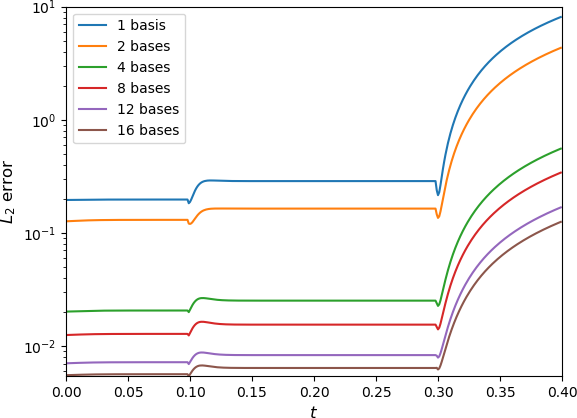
\includegraphics[width=0.45\linewidth]{L2_log.png} 
\hspace{2em}
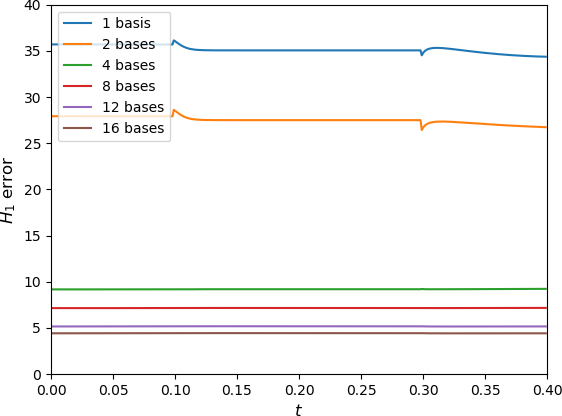
\includegraphics[width=0.45\linewidth]{H1.png} 
\caption{Relative $L_2$ and $H_1$ errors ($\%$) of the multiscale solution.}
\label{p5}
\end{figure} 

In Table~\ref{t2}, we present relative $L_2$ and $H_1$ errors at final time for different number of multiscale basis functions.
For example, when we use 8 spectral basis functions, we obtain $0.34\%$ $L_2$ error and $7.18\%$ $H_1$ error. 
Our comparison showed that it is prefer to use 4 or higher count of bases. 
The solution of the problem on a fine grid and multiscale solution using 16 basis functions on each local domain $\omega_i$ are shown in Figure \ref{p6}. Relative errors are 0.13\% for $L_2$ and 4.43\% for $H_1$. 

\begin{table}[h!]
\caption{Relative $L_2$ and $H_1$ errors ($\%$) of the solution at final time.}
\label{t2}
\begin{center}
\begin{tabular}{|c|c|r|r|r|}
\hline
Number of bases & Number of DOF & $L_2$ error & $H_1$ error & Calc time\\
\hline
1 & 49 & 8.09 & 34.36 & 0.015 \\
2 & 98 & 4.32 & 26.73 & 0.018 \\
4 & 196 & 0.56 & 9.24 & 0.026 \\
8 & 392 & 0.34 & 7.18 & 0.056 \\
12 & 588 & 0.17 & 5.17 & 0.102 \\
16 & 784 & 0.13 & 4.43 & 0.239 \\
fine & 115891 & -- & -- & 6.816 \\
\hline
\end{tabular}
\end{center}
\end{table}

\begin{figure}[h!]
\centering
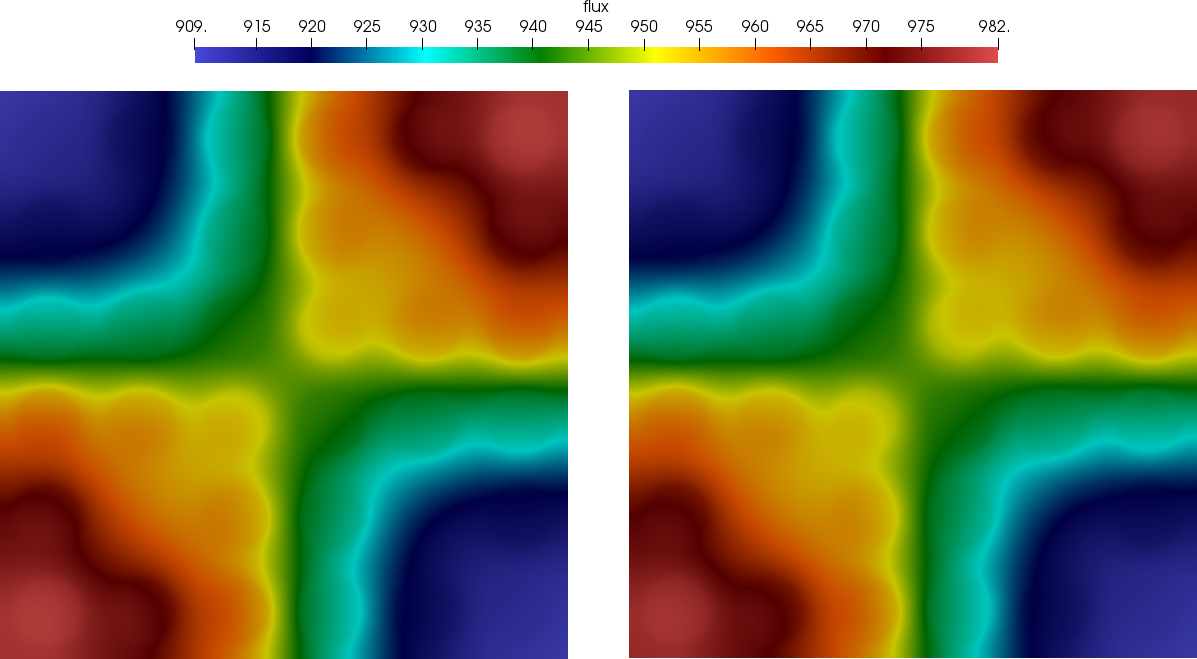
\includegraphics[width=0.75\linewidth]{flux.png} 
\caption{Fine grid and multiscale solution with 16 basis functions at final time.}
\label{p6}
\end{figure} 

\section{Conclusions}
A Generalized Multiscale Finite Element method was developed successfully for solving neutron diffusion in one-group approxmimation.  
We presented an implementation of GMsFEM. 
We considered each step of GMsFEM algorithm.
The results showed that GMsFEM has good accuracy in all cases.

In the current work, we considered the most popular and simplest model of neutron transport equation.
Computational expenses are always an issue even for modern computers.
In the future, we will consider more complex models of the neutron diffusion and transport equation such as $SP_3$ approximation. 

\section*{Acknowledgements}
This work was supported by the grant of the Russian Federation Government
(\#14.Y26.31.0013) and the Russian Science Foundation (\#19-71-00008).

\begin{thebibliography}{8}

\bibitem{Annals17}
Avvakumov, A.V., et al.: Spectral properties of dynamic processes in a nuclear reactor. Annals of Nuclear Energy. \textbf{99}, 68--79 (2017) 

\bibitem{Progress18}
Avvakumov, A.V., et al.: State change modal method for numerical simulation of dynamic processes in a nuclear reactor. Progress in Nuclear Energy. \textbf{106}, 240--261 (2018)

\bibitem{Duderstadt1976}
Duderstadt, J.J., Hamilton, L.J.: Nuclear Reactor Analysis. Wiley (1976)

\bibitem{dulla2008quasi}
Dulla, S., Mund, E.H., Ravetto, P.: The quasi-static method revisited. Progress in Nuclear Energy \textbf{50}(8), 908--920 (2008)

\bibitem{Spiridonov2019}
Spiridonov, D., Vasilyeva, M., Leung, W.T.: A Generalized Multiscale Finite Element Method (GMsFEM) for perforated domain flows with Robin boundary conditions. Journal of Computational and Applied Mathematics. \textbf{357}, 319--328 (2019)

\bibitem{Stacey2007}
Stacey, W.M.: Nuclear Reactor Physics. Wiley (2007)

\bibitem{Stalnov2017}
Stalnov, D.A., Vasilyeva, M.V.: Numerical averaging for the heat conduction problem in inhomogeneous and perforated media. Herald of the Northeastern Federal University. MK Ammosov. \textbf{2}(58) (2017)

\bibitem{Bakhvalov2012}
Bakhvalov, N.S., Panasenko, G.: Homogenisation: averaging processes in periodic media: mathematical problems in the mechanics of composite materials. Springer Science
\& Business Media.  \textbf{36} (2012)

\bibitem{Efendiev2009}
Yalchin, E., Thomas, Y.H.: Multiscale finite element methods: theory and applications.
Springer Science \& Business Media. \textbf{4} (2009)

\end{thebibliography}
\end{document}
